\documentclass[10pt,a4paper]{article}
% for margining standards
\usepackage[left=3cm,right=3cm,top=3cm,bottom=3cm]{geometry}
% for counting references as a section
\usepackage[numbib,notlof,notlot,nottoc]{tocbibind}
% useful packages
\usepackage{
                graphicx, setspace, fontspec, caption,
                subcaption, float, polyglossia, rotating,
                lscape, pdflscape, indentfirst, tocloft,
                multirow, amsmath, currfile
            }
% paragraph related package
\usepackage[parfill]{parskip}
% use bzar font(THIS MUST BE LOADED BEFORE XePerian PACKAGE)
\setmainfont{BZar.ttf}
% the dear XePersian package
\usepackage{xepersian}
%
% General settings goes here.
%
% lines space
\renewcommand{\baselinestretch}{1.5}
% paragraph first line indention
\setlength{\parindent}{1cm}
% paragraph spacing
\setlength{\parskip}{1em}
% set graphics' path
\graphicspath{ {images/} }
% make table of content dotted
\renewcommand{\cftsecleader}{\cftdotfill{\cftdotsep}}
% define a new command as {half-space} in english
\newcommand{\halfspace}{\hspace{0pt}}
% define a new command as {half-space} in persian
\newcommand{\نیمفاصله}{\halfspace}
% define a shortcut for half-space in general
\renewcommand{\ }{\halfspace}
% define a new command for ease of use for rendering reference
\newcommand{\renderref}[1] { \begingroup \let\clearpage\relax \include{#1} \endgroup }
%
% DOCUMENT BEGIN
%
\begin{document}
\title{گزارش پروژه\ ی پایان\ نیم سال درس رباتیک}
\author{داریوش حسن\ پور آده}
\date{۹۳۰۸۱۶۴}
\maketitle
\null
\vfill
\newpage
\قسمت{مقدمه}
طبق تعریف اولیه پروژه مبنی بر تعمییر و راه\ اندازی ربات مین\ یاب آزمایشگاه هوش\ مصنوعی به علت محدودیت\ های سخت افزاری/معماری ربات مذکور و عدم امکان \تاکید{مانورو} برای پیاده\ سازی حداقل یکی از الگوریتم\ های درس رباتیک بروی ربات پروژه ی ثانویه جهت شبیه\ سازی رفتار ربات در صورتی که ربات توانایی سرعت\ دهی دلخواه به موتورهای خود را داشته باشد تخصیص داده شد. که در این گزارش به شرح هر یک از دو پروژه\ ی انجام شده می\ پردازیم.
\tableofcontents
\newpage
\قسمت{تعمییر و راه اندازی سخت\ افزاری ربات}
\زیرقسمت{سخت\ افزارهای ربات}
این ربات که در شکل
\ref{fig:ساختار-ربات}
نمایش ساختاری ربات آمده است؛ دارای مشخصات سخت\ افزاری زیر بوده است:\بند
{
    \setstretch{0}
    \begin{itemize}
        \item ۱ عدد شاسی
        \item ۴ عدد موتور
        \item ۴ عدد چرخ سوئدی (با $\gamma = \frac{\pi}{2}$)
        \item ۴ عدد سنسور مادون\ قرمز با حساسیت ۱۰ سانتی متر
        \item ۱ عدد برد
        \item ۲ عدد زیرپردازنده
        \item ۱ عدد نمایشگر با آدرس\ دهی ۴ بیتی
        \item ۱ عدد حسگر فلزیاب (معیوب)
    \end{itemize}
}
\begin{figure}[H]
    \centering
    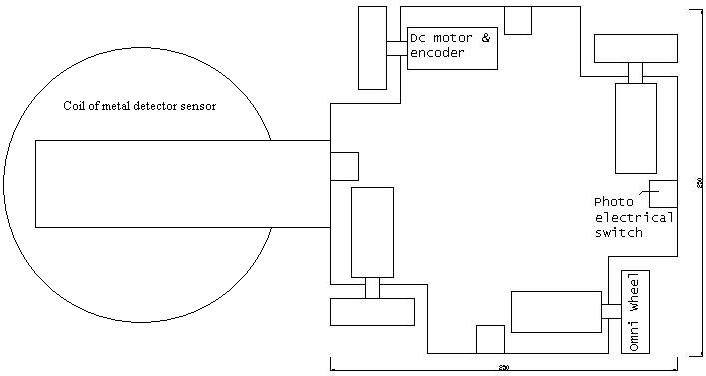
\includegraphics[width=1\textwidth]{deminer-structure}
    \caption{نمایش ساختاری ربات}
    \label{fig:ساختار-ربات}
\end{figure}
\زیرقسمت{شرح عملکرد ربات}
این ربات دارای ۴ چرخ دیفرانسیلی می\ باشد و هریک از چرخ\ های میتواند به صورت جدا دستورات سرعت متفاوتی را اجرا کنند ولی متاسفانه سازندگان این ربات مدارها را طوری سیم پیچی کرده اند که هر یک از چرخ\ ها میتواند فقط ۱ سرعت بگیرند(یا حرکت می\ کنند یا حرکت نمی\ کنند!) بنابراین امکان ایجاد حرکات زاویه دار که نیازمند تخصیص سرعت های متفاوتی به چرخ\ ها می\ باشند را ندارد.\بند
برای کنترل ربات یک ریزپردازنده
\lr{Atmega32}
استفاده شده است که تمامی سیگنال های حسگرها و دستورات کنترلی چرخ\ ها از طریق این ریزپردازنده کنترل میشوند. یک زیرپردازنده ی
\lr{Atmega8}
نیز برای انتزاع سازی علمیات مربوط به حسگر فلزیاب نیز تعبیه شده است که عملیات سطح پایین مربوط به راه\ اندازی, ارتباط و دریافت اطلاعات از حسگر فلزیاب را به عهده دارد و در انتها توسط یک وقفه به ریزپردانده اصلی(
\lr{Atmega32}
) فرستاده میشود که تشخیص فلز را اعلام می\ کند.
\زیرقسمت{شرح اتصالات اجزای الکترونیکی ربات}
همانطور که میدانیم ریزپردازنده ی
\lr{Atmega32}
دارای ۴ عدد درگاه\footnote{\lr{Port}}
با نام های انتزاعی
$A, B, C, D$
می\ باشد که هر یک دارای ۸ عدد اتصال\footnote{\lr{Pin}}
می\ باشند که در شکل
\ref{fig:شما-ربات}
 شمای کلی اتصالات ربات آمده است و در این قسمت به معرفی اتصالات این درگاه\ ها با سایر قسمت\ های مدار می\ پردازیم.
\begin{figure}[H]
    \centering
    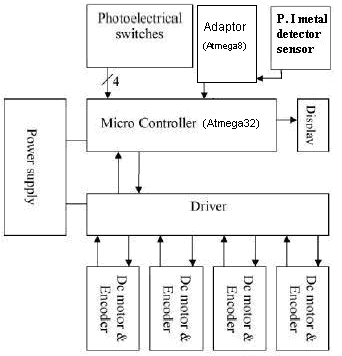
\includegraphics[width=0.5\textwidth]{deminer-schema}
    \caption{نمایش شماتیکی ربات}
    \label{fig:شما-ربات}
\end{figure}
\زیرزیرقسمت{اتصالات درگاه $A$}
درگاه $A$ اختصاصا برای اتصالات راه\ اندازه\زیرنویس{\lr{Driver}}های موتورها استفاده شده است. که به شرح جدول
\ref{table:درگاه A}
می\ باشد.
\begin{table}[H]
    \centering
    \begin{latin}
        \begin{tabular}{ |c|c|c| }
            \hline
            Pin &
            Connection &
            Target Motor\\
            \hline
            $A_0$ & Input 1 Of Driver 1 & \multirow{2}{*}{Motor 2}\\
            $A_1$ & Input 2 Of Driver 1 & \\
            \hline
            $A_2$ & Input 3 Of Driver 1 & \multirow{2}{*}{Motor 1}\\
            $A_3$ & Input 4 Of Driver 1 & \\
            \hline
            $A_4$ & Input 1 Of Driver 2 & \multirow{2}{*}{Motor 3}\\
            $A_5$ & Input 2 Of Driver 2 & \\
            \hline
            $A_6$ & Input 3 Of Driver 2 & \multirow{2}{*}{Motor 4}\\
            $A_7$ & Input 4 Of Driver 2 & \\
            \hline
        \end{tabular}
    \end{latin}
    \caption{مشخصات اتصالات درگاه \lr{A}}
    \label{table:درگاه A}
\end{table}
\زیرزیرقسمت{اتصالات درگاه $B‌$}
این درگاه برای کار با حسگرهای مادون\ قرمز مورد استفاده قرار گرفته اند. که شامل اتصالات $2, 1, 0$ و ۳ می\ باشند که به ۴ حسگر بعنوان ورودی حسگرها فرستاده شده است.
\زیرزیرقسمت{اتصالات درگاه $C$}
از اتصالات درگاه $C$ فقط اتصالات ۰ و ۲ برای بازنشانی و فعال کردن نمایشگر استفاده شده است.
\زیرزیرقسمت{اتصالات درگاه $D$}
اتصالات درگاه $D$ به صورت جدول
\ref{table:درگاه D}
است.
\vspace{-0.2em}
\begin{table}[H]
    \centering
    \begin{latin}
        \begin{tabular}{ |c|c|c| }
            \hline
            Pin &
            Connection &
            Description \\
            \hline
            $D_0$ & {\small NOT USED} & \multirow{2}{*}{N/A}\\
            $D_1$ & {\small NOT USED} & \\
            \hline
            $D_2$ & Sensor Input 0-2 & \multirow{2}{*}{Interrupt}\\
            $D_3$ & Sensor Input 1-3 & \\
            \hline
            $D_4$ & LCD Output & \multirow{4}{*}{Mapped accordingly to LCD's PortC4{\ldots}7}\\
            $D_5$ & LCD Output & \\
            $D_6$ & LCD Output & \\
            $D_7$ & LCD Output & \\
            \hline
        \end{tabular}
    \end{latin}
    \caption{مشخصات اتصالات درگاه \lr{D}}
    \label{table:درگاه D}
\end{table}
توجه شود که علت اینکه ۲ عدد وقفه برای ۴ عدد حسگر استفاده شده است این است که هر ۲ حسگر جلو و عقب به یک اتصال وقفه می\ دهند و بدین صورت که در حالت عادی فقط یکی از این حسگرها عمل میکنند و براحتی از سرعت چرخ\ ها میتوان حدس زد که کدام حسگر وقفه را ارسال کرده است و همین مساله برای حسگرهای چپ و راست نیز صادق است.
\زیرزیرقسمت{برنامه\ ریزی ربات}
برای برنامه\ ریزی ربات و کنترل ربات فقط کافی است که ریزپردازنده
\lr{Atmega32}
را برنامه ریزی نمیاییم. که برنامه ی نوشته شده به زبان
\lr{AVR}
بوده و توسط کامپایلر
\lr{avr-gcc (GCC) 4.8.2}
تحت سیستم عامل 
\lr{Linux 3.13.0-34-generic}
کامپایل گردیده است
 و توسط
\lr{avrdude 6.0.1}
 به داخل ریزپردازنده سوخته\زیرنویس{\lr{Burn}} شده است. که توضیح راجع به روند سوزاندن و کدهای سوخته شده خارج از حوصله ی این نوشتار است.
\قسمت{شبیه\ سازی نرم\ افزاری ربات}
برای پیاده\ سازی شبیه\ سازی مورد نیاز برای هدایت روبات به مختصات دلخواه نیاز به نوشتن روابط سینماتیکی مورد نیاز داریم.\
\cite{IAMR}
برای نوشتن روابط سینماتیکی ربات ابتدا باید آنرا مدل\ سازی کنیم.
\زیرقسمت{مدل\ سازی ریاضی ربات}
 برای مدل\ سازی اینطور در نظر گرفتیم که هر چرخ با چرخ دیگر دارای اختلاف درجه  $\frac{\pi}{2}$ بوده است و با هر یک از محورهای محلی خود دارای زاویه $\frac{\pi}{4}$ هستند. که در شکل
\ref{fig:مدل-ربات}
آمده است. همانطور که در شکل
\ref{fig:مدل-ربات}
میبینید جهت چرخش  \textbf{مثبت} چرخ\ ها آمده است و چرخ\ ها به ترتیب نواحی مثلثاتی که در آن قرار دارند شماره گذاری شده اند.
\begin{figure}[H]
    \centering
    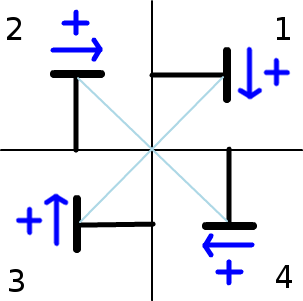
\includegraphics[width=0.25\textwidth]{deminer-model}
    \caption{نمایش مدلی ربات برای شبیه\ سازی ربات در متلب}
    \label{fig:مدل-ربات}
\end{figure}
برای بدست\ آوردن محدودیت\ های سینماتیکی تحمیل شده از طرف چرخ\ ها نیاز داریم ویژگی های هندسی چرخ\ ها را معین کنیم که در جدول
\ref{table:مشخصات هندسی چرخ ها}
آمده است. در جدول
\ref{table:مشخصات هندسی چرخ ها}
مقادیر $r$ و $l$ را باتوجه به مقادیر داده شده به تمرین دوم این درس در نظر گرفته شده\ اند.
\begin{table}[H]
    \centering
    \begin{latin}
        \begin{tabular}{ |p{1.5cm}|c|c|c|c|c| }
            \hline
            Wheel\# &
            $\alpha$ &
            $\beta$  &
            $\gamma$ &
            $l$      &
            $r$      \\
            \hline
            1 & $\frac{\pi}{4}$  & $-\frac{\pi}{4}$ & $\frac{\pi}{2}$ & {\small 0.25 } & {\small 0.125}\\
            \hline
            2 & $\frac{3\pi}{4}$ & $-\frac{\pi}{4}$ & $\frac{\pi}{2}$ & {\small 0.25 } & {\small 0.125}\\
            \hline
            3 & $\frac{5\pi}{4}$ & $-\frac{\pi}{4}$ & $\frac{\pi}{2}$ & {\small 0.25 } & {\small 0.125}\\
            \hline
            4 & $\frac{7\pi}{4}$ & $-\frac{\pi}{4}$ & $\frac{\pi}{2}$ & {\small 0.25 } & {\small 0.125}\\
            \hline
        \end{tabular}
    \end{latin}
    \caption{مشخصات هندسی چرخ\ ها}
    \label{table:مشخصات هندسی چرخ ها}
\end{table}
با توجه به رابطه\ ی
\ref{eq:معادله کلی محدودیت سینماتیکی}
که بیانگر رابطه\ ی محدودیت\ های اعمال شده توسط چرخ\ های ثابت و فرمان\ پذیر استاندارد به ربات می\ باشد و با توجه به داده\ ی موجود در جدول
\ref{table:مشخصات هندسی چرخ ها}
به محاسبه\ ی عناصر رابطه\ ی
\ref{eq:معادله کلی محدودیت سینماتیکی}
در معادلات
\ref{eq:J1}\ldots\ref{eq:phidot}
می\ پردازیم.
    \begin{equation}
        J_1R(\theta)\dot{\xi}_I = J_2\dot{\phi}
        \label{eq:معادله کلی محدودیت سینماتیکی}
    \end{equation}
    \begin{equation}\small
    J_1 = \begin{bmatrix}
            \sin{(\alpha_1 + \beta_1 + \gamma_1)} & -\cos{(\alpha_1 + \beta_1 + \gamma_1)} & -l_1\cos{(\beta_1 + \gamma_1)}\\
            \sin{(\alpha_2 + \beta_2 + \gamma_2)} & -\cos{(\alpha_2 + \beta_2 + \gamma_2)} & -l_2\cos{(\beta_2 + \gamma_2)}\\
            \sin{(\alpha_3 + \beta_3 + \gamma_3)} & -\cos{(\alpha_3 + \beta_3 + \gamma_3)} & -l_3\cos{(\beta_3 + \gamma_3)}\\
            \sin{(\alpha_4 + \beta_4 + \gamma_4)} & -\cos{(\alpha_4 + \beta_4 + \gamma_4)} & -l_4\cos{(\beta_4 + \gamma_4)}\\
    \end{bmatrix} = \begin{bmatrix}
    0    &    -1    &    -0.1768\\
    1    &    -0    &    -0.1768\\
    0    &    +1    &    -0.1768\\
   -1    &    +0    &    -0.1768\\
    \end{bmatrix}
    \label{eq:J1}
    \end{equation}
    \begin{equation}\small
    R(\theta) = \begin{bmatrix}
    \cos{(\theta)} & \sin{(\theta)} & 0\\
    -\sin{(\theta)} & \cos{(\theta)} & 0\\
    0 & 0 & 1
    \end{bmatrix}
    \label{eq:Rtheta}
    \end{equation}
    \begin{equation}
    \dot{\xi}_I = \begin{bmatrix}
        \dot{x} &
        \dot{y} &
        \dot{\theta}
    \end{bmatrix} ^ T
    \label{eq:xidor}    
    \end{equation}
    \begin{equation}\small
    J_2 = \begin{bmatrix}
    {\small 0.125} & 0 & 0 & 0\\
    0 & {\small 0.125} & 0 & 0\\
    0 & 0 & {\small 0.125} & 0\\
    0 & 0 & 0 & {\small 0.125}\\
    \end{bmatrix} 
    \label{eq:J2}    
    \end{equation}
    \begin{equation}
    \dot{\phi} = \begin{bmatrix}
        \dot{\phi_1} &
        \dot{\phi_2} &
        \dot{\phi_3} &
        \dot{\phi_4}
    \end{bmatrix} ^ T
    \label{eq:phidot}
    \end{equation}
که با انتقال معلومات معادله\ ی
\ref{eq:معادله کلی محدودیت سینماتیکی}
 به سمت راست رابطه و جایگذاری معادلات
\ref{eq:J1}\ldots\ref{eq:phidot}
در معادله\ ی
\ref{eq:معادله کلی محدودیت سینماتیکی}
 و اعمال عملیات ریاضی مورد نیاز بروی مقادیر ثابت معادله، به معادله\ ی
\ref{eq:معادله ی نهایی محدودیت های سینماتیک}
میرسیم.
\begin{equation}\small
\dot{\xi}_I(\phi_{1\ldots4}, \theta) = \begin{bmatrix}
    \cos{(\theta)} & -\sin{(\theta)} & 0\\
    \sin{(\theta)} & \cos{(\theta)} & 0\\
    0 & 0 & 1
\end{bmatrix} * \begin{bmatrix}
    0.0000  & +0.0625  &  +0.0000  &  -0.0625\\
   -0.0625  & -0.0000  &  +0.0625  &  -0.0000\\
   -0.1768  & -0.1768  &  -0.1768  &  -0.1768\\
\end{bmatrix} * \begin{bmatrix}
    \dot{\phi_1}\\
    \dot{\phi_2}\\
    \dot{\phi_3}\\
    \dot{\phi_4}\\
\end{bmatrix}
\label{eq:معادله ی نهایی محدودیت های سینماتیک}
\end{equation}
که معادله ی
\ref{eq:معادله ی نهایی محدودیت های سینماتیک}
با جایگذاری زاویه\ ی کنونی\ ای که ربات دارد و سرعت تک\ تک چرخ\ ها و اعمال عملیات ضرب\ ها سرعت لحظه\ ای ربات در مختصات جهانی بدست خواهد آمد؛ و با انتگرال\ گیری از آن می\ توان موقعیت ربات را در مختصات جهانی بدست آورد.
 \زیرقسمت{درجه\ ی مانورپذیری ربات مدل\ سازی شده}
\label{ssec:درجه ی مانورپذیری}
با توجه به اینکه در مدل\ سازی نرم\ افزاری ربات بر\ عکس نمونه واقعی ساخته شده؛ این مهم در نظر گرفته شده است که می شود به چرخ\ های مختلف سرعت\ های مختلف تخصیص داد(همان\ طور که معادله\ ی
\ref{eq:معادله ی نهایی محدودیت های سینماتیک}
پیشنهاد میدهد) لازم دانستم که اندکی در مورد درجه\ ی مانورپذیری ربات بحثی کنم تا در مورد نتایج حاصل از شبیه\ ساز ربات(که در قسمت
\ref{sec:نتیجه}
ارائه میشود) ابهامات احتمالی برطرف گردد.\بند
همانطور که میدانیم درجه\ ی مانورپذیری ربات($\delta_M$) از رابطه\ ی
\ref{eq:درجه ی مانورپذیری}
بدست می آید که برابر با مجموع درجات فرمان\ پذیری و تحرک ربات است. از آنجایی که این ربات هیچ چرخ فرمان\ پذیری ندارد بنابراین درجه\ ی فرمان\ پذیری آن صفر بوده است و بدیهی است که درجه\ ی تحرک\ ای برابر با مقدار ۳ دارد؛ بنابراین درجه\ ی مانورپذیری برابر ۳ دارد و میتواند در هر موقعیتی خود را قرار دهد.
\begin{equation}
\delta_M = \delta_m + \delta_s
\label{eq:درجه ی مانورپذیری}
\end{equation}
\زیرقسمت{کنترل ربات برای رسیدن به مختصات مشخص}
همانطور که در قسمت
\ref{ssec:درجه ی مانورپذیری}
بحث شد این ربات میتواند با تنظیم مناسب چرخ\ های خود در هر موقعیتی خود را قرار دهد. کنترل پیاده\ سازی شده برای کنترل سرعت و درجه ربات از ۲ مرحله تشکیل شده است که ابتدا ربات با همان زاویه در حال حاضر قرار دارد خود را به موقعیت مورد نظر برساند و سپس در موقعیت هدف زاویه خود را تغییر دهد -- در صورت انحراف از نقطه\ ی هدف در مرحله ۲ با استفاده از روند مرحله ی ۱ موقعیت خود را تصحیح کند سپس مرحله ۲ را ادامه دهد. که سرعت\ های هر یک از چرخ\ ها توسط معادله
\ref{eq:تخصیص سرعت}
تخصیص داده میشود.
\begin{equation}
\begin{bmatrix}
\dot{\phi_1}^\prime\\
\dot{\phi_2}^\prime\\
\dot{\phi_3}^\prime\\
\dot{\phi_4}^\prime\\
\end{bmatrix} = \begin{bmatrix}
-(K_{\rho} + K_{\epsilon})\sin{(\theta^\prime)}\\
+(K_{\rho} + K_{\epsilon})\cos{(\theta^\prime)}\\
+(K_{\rho} + K_{\epsilon})\sin{(\theta^\prime)}\\
-(K_{\rho} + K_{\epsilon})\cos{(\theta^\prime)}\\
\end{bmatrix}
\label{eq:تخصیص سرعت}
\end{equation}
که در معادله
\ref{eq:تخصیص سرعت}
مقادیر
$K_{\rho}$
و $\theta^\prime$ توسط
\ref{eq:krho}
و
\ref{eq:thetaprim}
بدست می\ آیند.
\begin{equation}
K_{\rho} = \sqrt{\Delta{x}^2 + \Delta{y}^2}
\label{eq:krho}
\end{equation}
\vspace{-4.5em}
\begin{equation}
\theta^\prime = \arctan2{(\Delta{y}, \Delta{x})}
\label{eq:thetaprim}
\end{equation}
که در معادله ی
\ref{eq:تخصیص سرعت}
عبارت
$K_\epsilon$
برابر با یک مقدار دلخواه برای عادی\ سازی/بهینه\ سازی مقادیر
$K_\rho$
در برخی موارد خواص(معمولا مقداری برابر با صفر دارد) می باشد.
و
در معادلات
\ref{eq:krho}
و
\ref{eq:thetaprim}
منظور از
$\Delta{x}$
و
$\Delta{y}$
فاصله\ ی مولفه\ های دکارتی موقعیت کنونی ربات با موقعیت هدف می\ باشند. که بلوک-دیاگرام سیمولینک شبیه\ ساز در شکل
\ref{fig:سمولینک-ربات}
آورده شده است.
\vspace{-1em}
\begin{figure}[H]
    \centering
    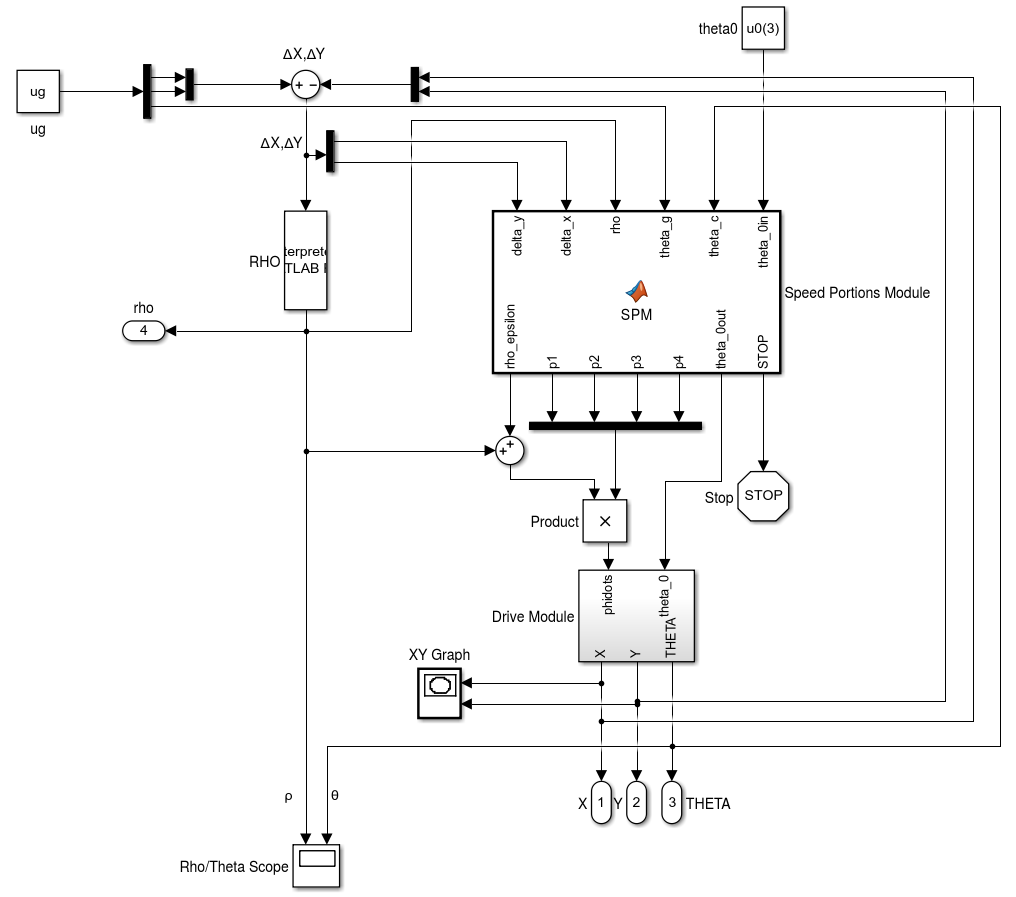
\includegraphics[width=1\textwidth]{deminer-simu}
    \caption{بلوک-دیاگرام پیاده\ سازی شده در شبیه\ ساز}
    \label{fig:سمولینک-ربات}
\end{figure}
\قسمت{نتیجه}
\label{sec:نتیجه}
در شکل
\ref{fig:نتیجه-سمولینک-ربات}
نتیجه یک نمونه اجرا آورده شده است که در این نمونه اجرا از ربات خواسته شده است که از موقعیت
\lr{$\begin{bmatrix}
3 & -2 & \frac{3\pi}{2}
\end{bmatrix}^T$}
خود را به موقعیت
\lr{$\begin{bmatrix}
-4 & 0 & \frac{\pi}{2}
\end{bmatrix}^T$}
برساند.
\begin{figure}[H]
    \centering
    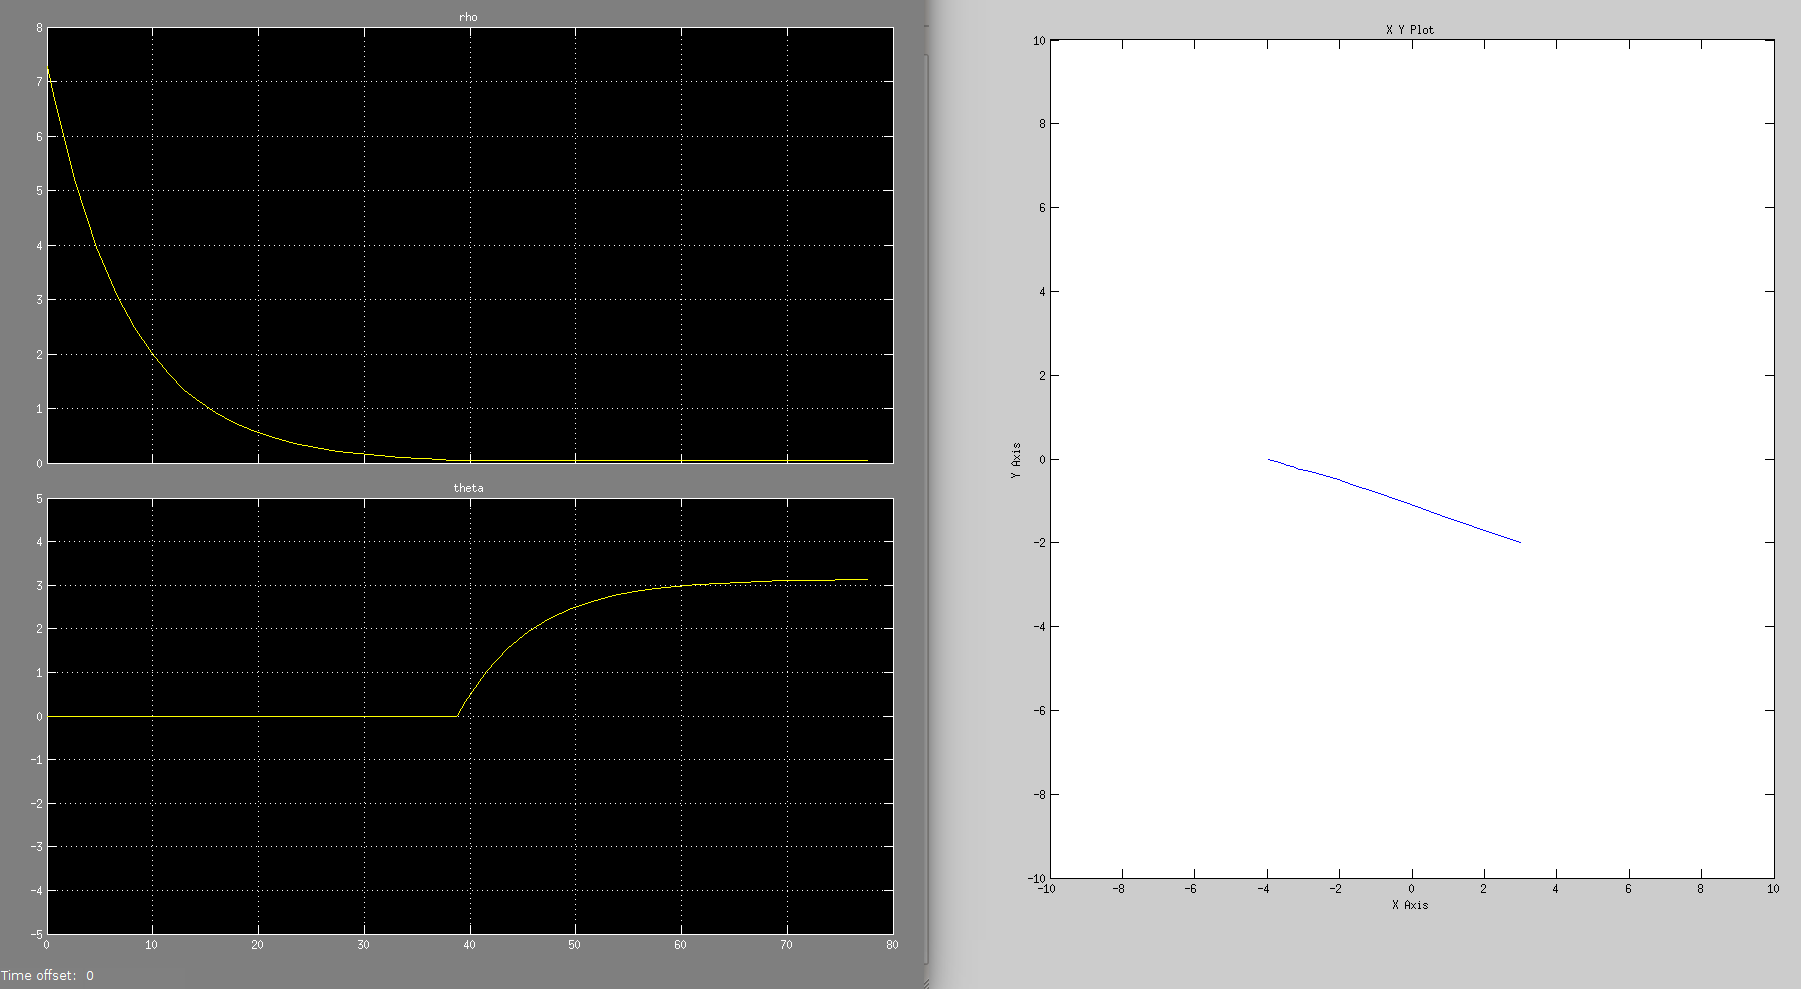
\includegraphics[width=1\textwidth]{deminer-simu-result}
    \caption{نتیجه یک نمونه اجرای بلوک-دیاگرام شکل
\ref{fig:سمولینک-ربات}
که از ربات خواسته شده است که موقعیت کنونی\ اش خود را به موقعیت هدفش برساند.     
    }
    \label{fig:نتیجه-سمولینک-ربات}
\end{figure}
که همانطور که در شکل
\ref{fig:نتیجه-سمولینک-ربات}
سمت راست میبینید ربات براحتی توانسته با یک مسیر مستقیم خود را به هدف برساند. در شکل
\ref{fig:نتیجه-سمولینک-ربات}
سمت چپ ابتدا ربات به کاهش فاصله\ اش با هدف(چپ-بالا) میپردازد پس از آنکه به موقعیت هدف رسید به تغییر زاویه\ ی خود(چپ-پایین) به زاویه\ ی دلخواه می\ رساند؛ که شکل سمت چپ-یایین میزان تغییرات زاویه انجام شده را نشان می\ دهد -- که در ابتدا میزان تغییرات زاویه صفر بوده و سپس به اندازه $+\pi^\circ$ تغییر زاویه داده است(همانطور که انتظار میرفت).
\section{مراجع}
\renderref{reference}
\end{document}